\documentclass[11pt]{article}
\newcommand{\thetitle}{HYPERION Memo \#3: Testing the Radio Environment in 
Rangely, CO}
\newcommand{\theauthor}{Kara Kundert and Raj Biswas}
\newcommand{\theauthorsemail}{kkundert@berkeley.edu, rbiswas@berkeley.edu}
\newcommand{\thedate}{September 2017}
% the following controls some aspects of how the text is displayed on the page
\setlength{\textwidth}{6.5in}
\setlength{\textheight}{8.25in}
\setlength{\oddsidemargin}{0in}

% set up the page headers and footers
\usepackage{fancyhdr}
    \pagestyle{fancy}
    \lhead{\sffamily\slshape\small\thetitle}
    \rhead{\sffamily\small\theauthor}
    \cfoot{\sffamily\slshape\small\thepage}

% support display of graphics
\usepackage{graphicx}

% the following control some aspects of how paragraphs are displayed
\parindent=0pt
\parskip=2ex

% import library of technical symbols
\usepackage{amsmath,amssymb,latexsym}

% import bibliography tools
\usepackage{natbib}
\citestyle{aa}

\begin{document}
% print the title in san-serif font, in bold, in huge characters
\title{
    \sffamily\bfseries\huge
    \thetitle \\
}
% print the author in san-serif font
\author{
    \sffamily\theauthor \\
    \sffamily\theauthorsemail
}
\date{\thedate}
\maketitle
\sloppy

\section{Introduction}

This memo lays out the results of some initial radio environment testing in and 
around Rangely, Colorado. It also aims to lay out some analysis of what these 
results mean for the HYPERION instrument and suggests some new ideas for 
mitigation of environmental factors.

\section{Background and Theory}

\citep{pritchard-loeb2010}

\begin{equation}
    \label{eq:baffle-temp}
    T_{baffle} = T_{sky} * 10^{dB/10} + T_{abs} * (1 - 10^{dB/10})
\end{equation}

\section{Method}


\section{Data and Analysis}

\begin{figure}
    \begin{center}
    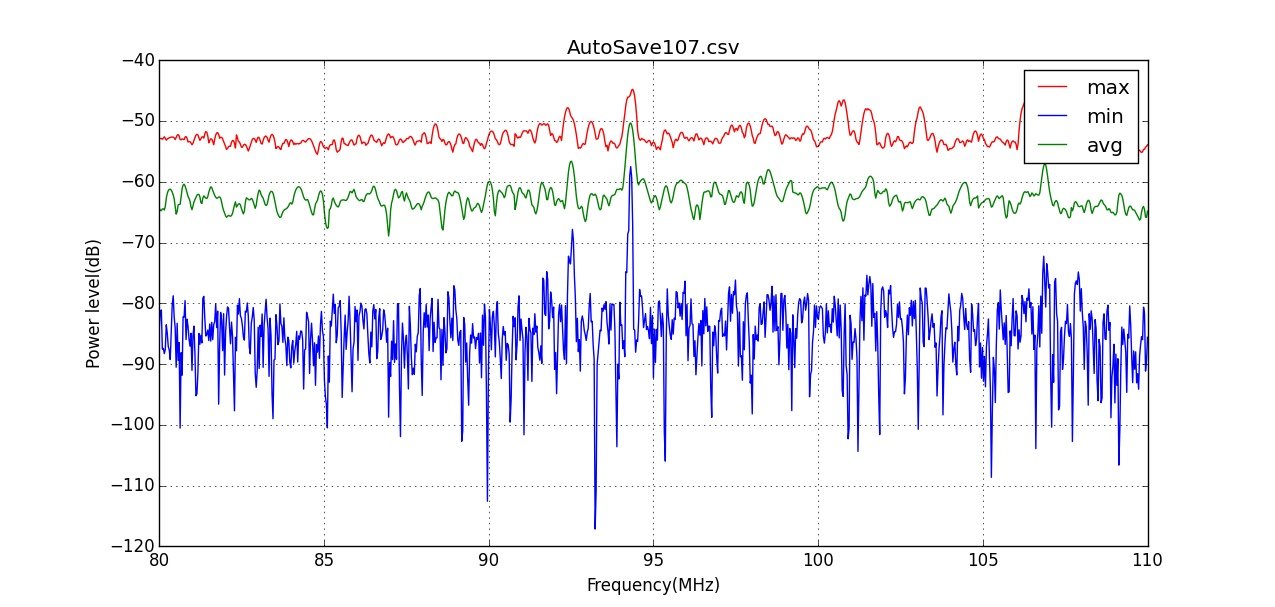
\includegraphics[width=\linewidth]{/home/kara/documents/hyperion/memos/memo3figs/107.jpeg}
    \end{center}
    \caption{
        Pictured above is the radio environment from 80-110 MHz as measured 
        from the creek bed in the box canyon off of Cottonwood Road, 
        approximately 15 miles southwest of Rangely.
    }
    \label{fig:sys-temp}
\end{figure}

\section{Conclusions}


\bibliography{hyperion}{}
\bibliographystyle{apj}

\end{document}





